\section{Related Works}

\begin{frame}{Problem Formulation}
    \begin{block}{Problem}
        Given a set of problems (software bugs) be denoted as \( P = \{P_1, P_2, \ldots, P_N\} \), where each problem \( P_i \) is associated with a description \( D_i \) detailing the observed errors.\\

        Additionally, for each problem \( P_i \), there exist multiple unit tests \( U_{i,j} \), the model has access to these unit tests to guide the correction process.\\
        \vspace{0.5cm}
        The goal is to maximize the \textbf{`pass@k'} metric, which is defined as the percentage of problems in the set for which the $k$ initial attempts at correction passes all associated unit tests successfully.
    \end{block}
\end{frame}

\begin{frame}{Taxonomy of Related Works}
    \begin{figure}
        \centering
        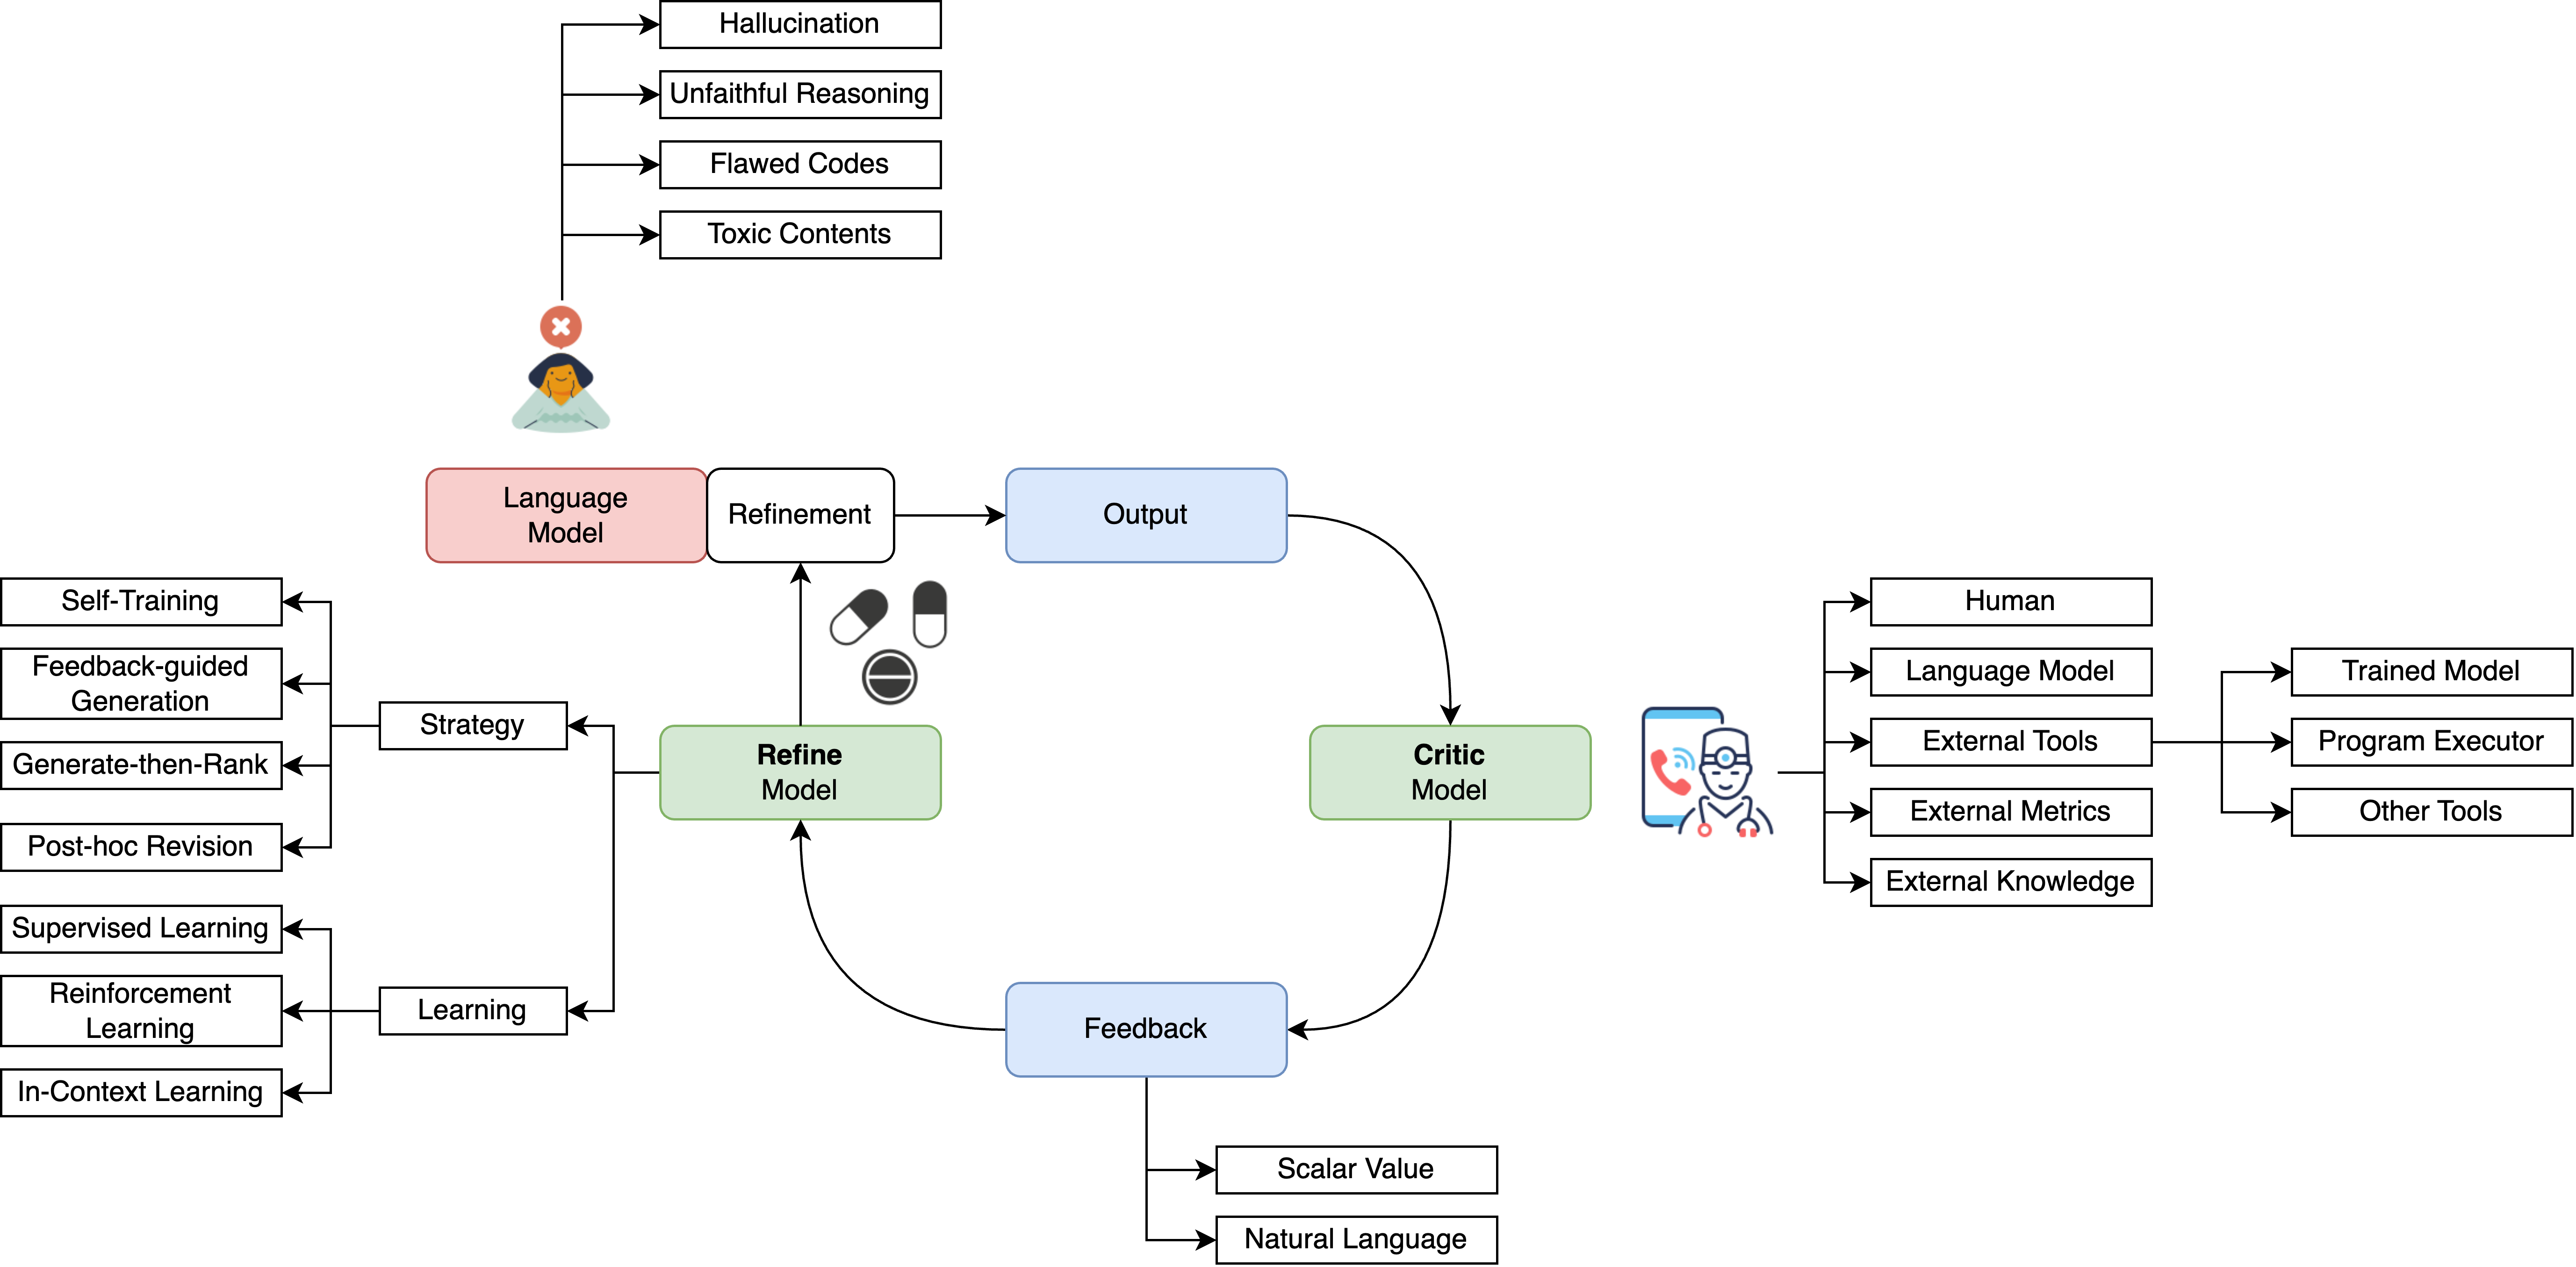
\includegraphics[width=1\textwidth]{img/taxonomy}
        \captionsetup{font=small,labelformat=empty}
        \caption{Taxonomy of related works.}\label{fig:taxonomy}
    \end{figure}
\end{frame}

% \begin{frame}{Language Model}
%     \begin{columns}[T]
%         \begin{column}{0.70\textwidth}
%             The works aimed at correcting LLMs can be classified according to the issues they tackle:
%             \begin{enumerate}
%                 \item Hallucination: plausible-sounding but false information~\cite{gao2023rarr, zhang2023language}.

%                 \item Unfaithful Reasoning: derived conclusion does not follow the previously generated reasoning chain~\cite{he2022rethinking, pan2023logiclm}.

%                 \item Toxic Contents: content that is toxic, biased, or harmful due to biases present in the training datas~\cite{lu2022quark, gou2023critic}.

%                 \item Flawed Codes: flawed or incorrect code generation~\cite{chen2023teaching, olausson2023selfrepair}.
%             \end{enumerate}
%         \end{column}
%         \begin{column}{0.30\textwidth}
%             \begin{figure}[!htb]
%                 \centering
%                 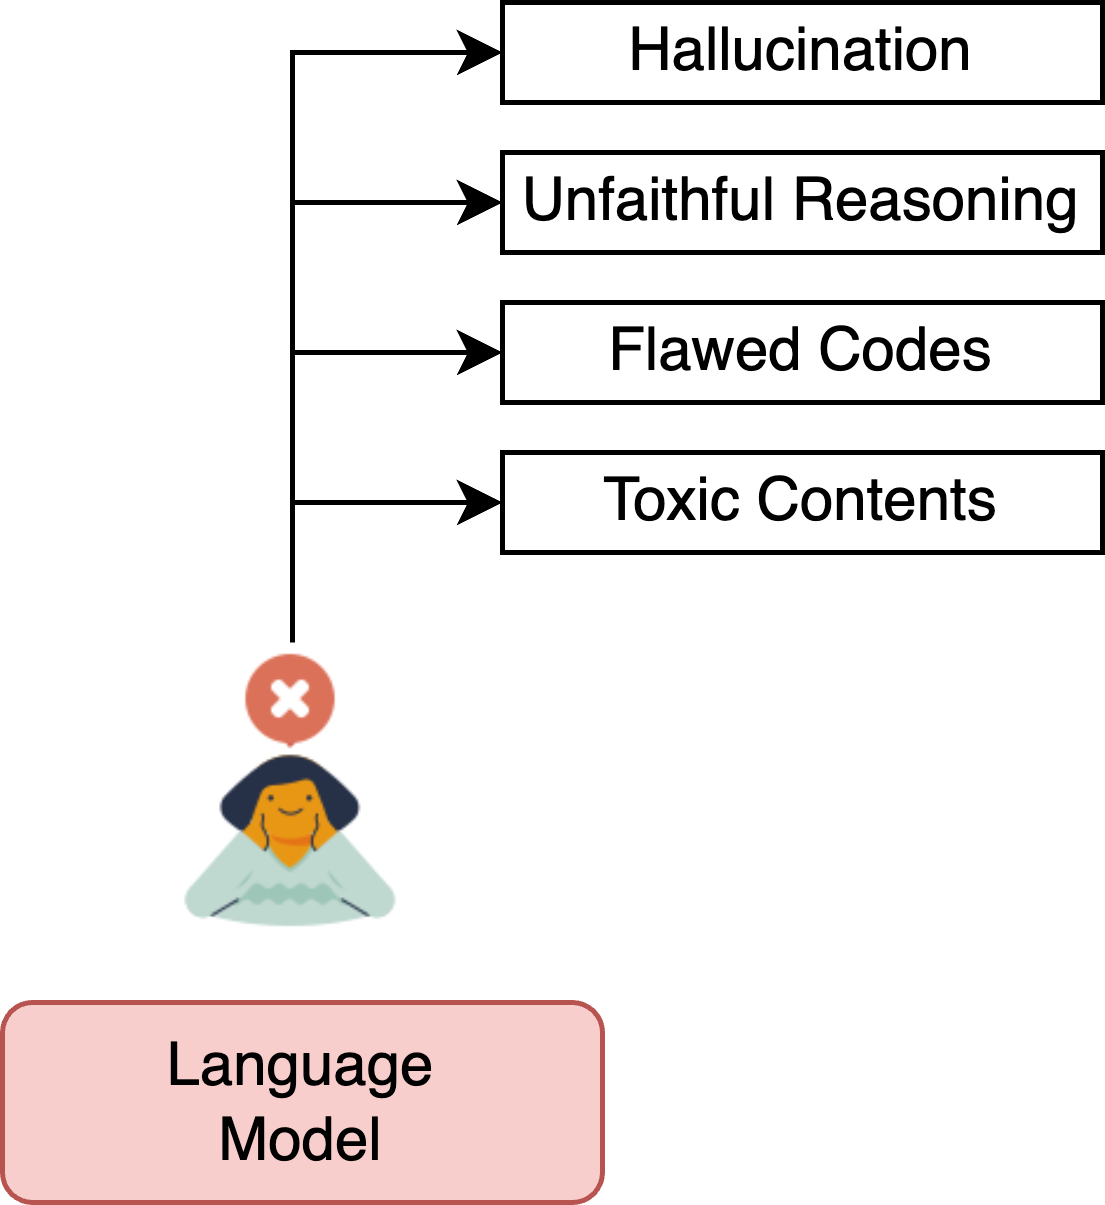
\includegraphics[width=1\textwidth]{img/language_model}
%                 \captionsetup{font=small,labelformat=empty}
%                 \caption{Problems of LLMs.}
%             \end{figure}
%         \end{column}
%     \end{columns}
% \end{frame}

% \begin{frame}{Critic Model}
%     \begin{columns}[T]
%         \begin{column}{0.55\textwidth}
%             Source of feedback:
%             \begin{enumerate}
%                 \item Self-Feedback: the model itself generates feedback~\cite{weng2023large}.

%                 \item External Feedback: the model receives feedback from an external source (e.g., human, program executor and external knowledge)~\cite{gou2023critic}.
%             \end{enumerate}

%             Format of feedback:
%             \begin{enumerate}
%                 \item Scalar Value: metrics based on pre-defined tests~\cite{weng2023large}.

%                 \item Natural Language: provides richer information than scalar value feedback~\cite{chen2023teaching}.
%             \end{enumerate}
%         \end{column}
%         \begin{column}{0.45\textwidth}
%             \begin{figure}[!htb]
%                 \centering
%                 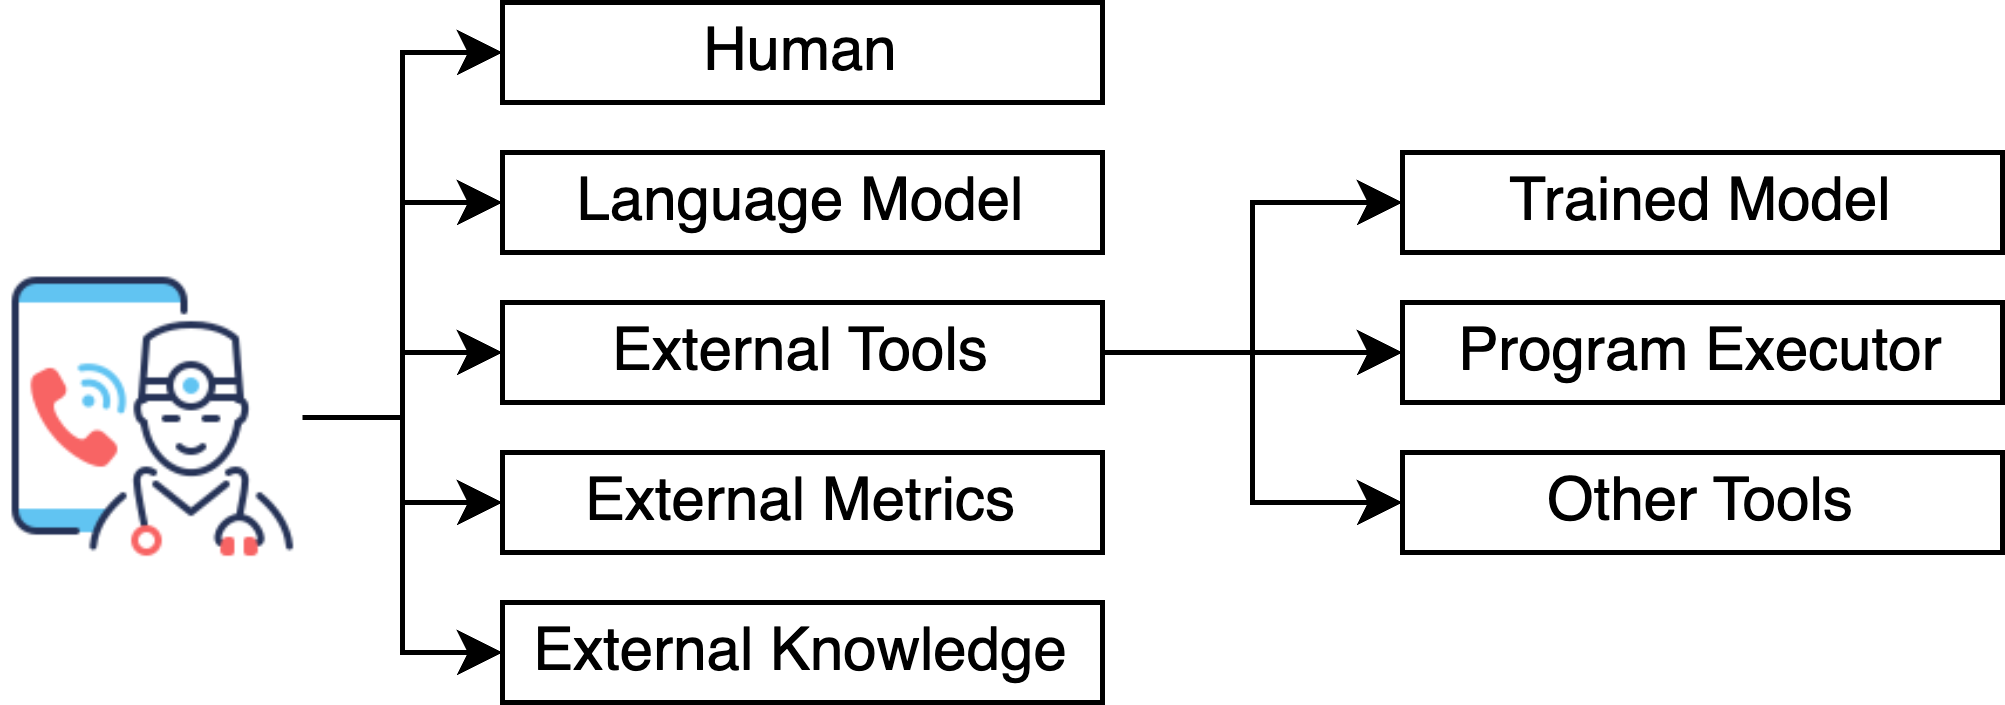
\includegraphics[width=1\textwidth]{img/critic_model}
%                 \captionsetup{font=small,labelformat=empty}
%                 \caption{Critic Model.}
%             \end{figure}
%         \end{column}
%     \end{columns}
% \end{frame}

% \begin{frame}{Refine Model}
%     The Refine Model is the most active area of research in the field. Existing works can be classified based on the following key questions:
%     \begin{enumerate}
%         \item Need to update the LLMs? \textbf{Yes}: Self-Training~\cite{huang2022large}, Supervised Learning~\cite{bai2022training}, Reinforcement Learning~\cite{dubois2024alpacafarm}, In-Context Learning~\cite{dong2022survey}.

%         \item When to refine: generation-time or post-hoc?
%               \begin{itemize}
%                   \item Generation-time: Generate-then-Rank~\cite{cobbe2021training}, Feedback-Guided Generation~\cite{yao2023tree}.
%                   \item Post-hoc: Models/Tools as Feedback~\cite{zhang2023selfedit}, Multi-Agent Debate~\cite{du2023improving}.
%               \end{itemize}
%     \end{enumerate}
% \end{frame}

\begin{frame}{Challenges and Opportunities}
    \begin{enumerate}
        \item The majority of existing LLMs are closed-sourced, such as OpenAI's GPT-4, or have an infeasibly large number of parameters for training within the scope of this research, such as the 70-billion parameter LLaMa model.

        \item The source code of common data science libraries like Pandas and Numpy is extensive, posing a challenge for LLMs to sufficiently capture the context of the full codebase.

        \item Although complex, software systems have structured and well-tested code, allowing the feedback from critic models to be reliable.
    \end{enumerate}
\end{frame}

\begin{frame}{Research Direction}
    \begin{figure}[!htb]
        \centering
        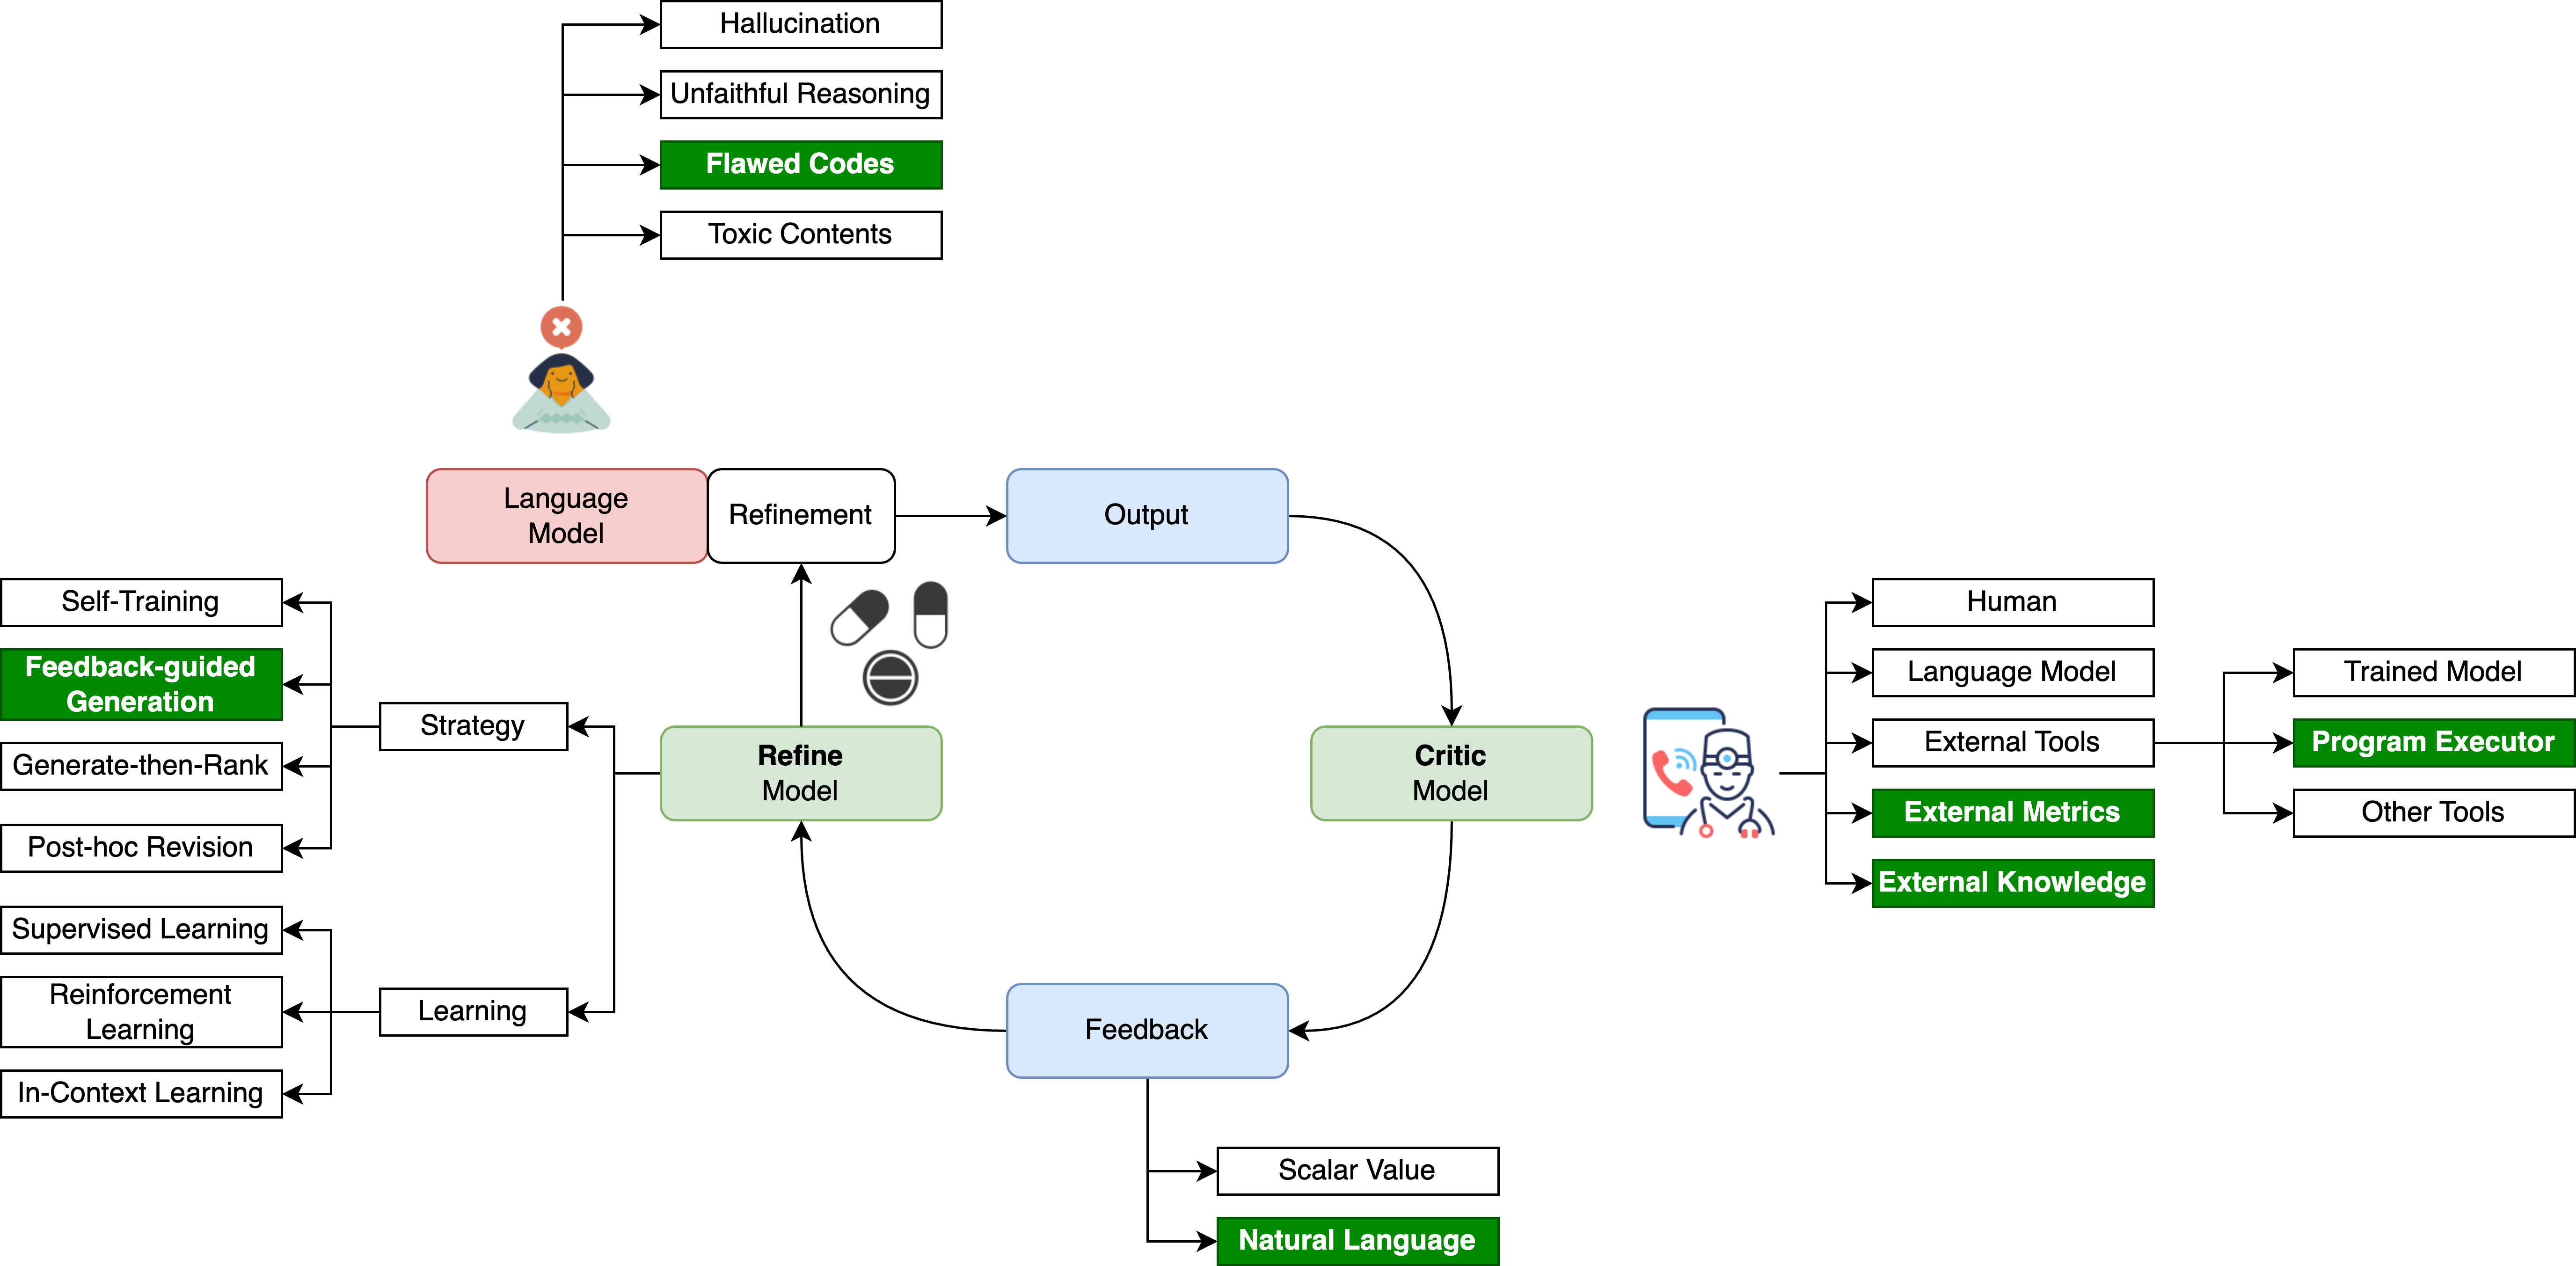
\includegraphics[width=1\textwidth]{img/direction_of_research}
        \captionsetup{font=small,labelformat=empty}
        \caption{Research Direction.}
    \end{figure}
\end{frame}
